% Created 2025-02-04 Tue 16:04
% Intended LaTeX compiler: pdflatex
\documentclass[11pt]{article}
\usepackage[utf8]{inputenc}
\usepackage[T1]{fontenc}
\usepackage{graphicx}
\usepackage{longtable}
\usepackage{wrapfig}
\usepackage{rotating}
\usepackage[normalem]{ulem}
\usepackage{amsmath}
\usepackage{amssymb}
\usepackage{capt-of}
\usepackage{hyperref}
\usepackage{listings}
\usepackage{algorithm}
\usepackage{algpseudocode}
\usepackage{amsmath}
\author{Akilan}
\date{\today}
\title{}
\hypersetup{
 pdfauthor={Akilan},
 pdftitle={},
 pdfkeywords={},
 pdfsubject={},
 pdfcreator={Emacs 29.1 (Org mode 9.6.6)}, 
 pdflang={English}}
\begin{document}

\tableofcontents


\section{Fat-pointer Address Translations}
\label{sec:orgda6e9a4}

Fat-pointer Address Translations, combined with the capabilities of the CHERI (Capability Hardware Enhanced RISC Instructions) 
architecture, introduce robust memory safety and security features by incorporating additional metadata 
with memory pointers. This enhanced architecture utilizes concepts such as FlexPointer, 
Range Memory Mapping (RMM) to manage memory effectively.

Range addresses play a pivotal role within this implementation, defining memory 
regions bounded by a starting address (Upper) and an ending address (Lower). 
These range addresses are encoded within FAT-pointers, allowing for precise 
control over memory regions.

\begin{figure}[htbp]
\centering
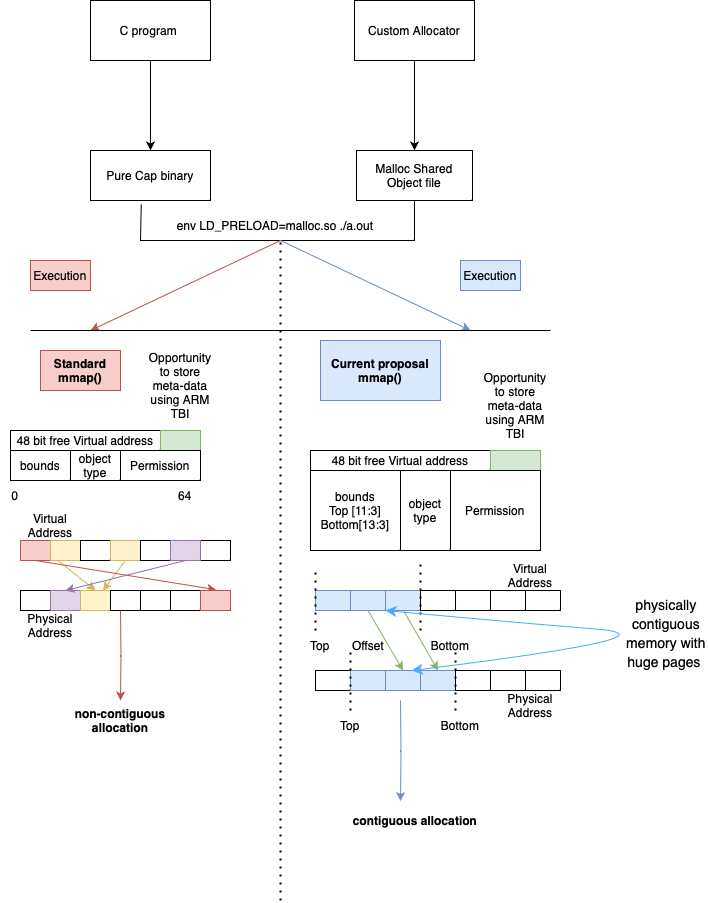
\includegraphics[width=.9\linewidth]{diagram/HighOverviewArchitecture24.png}
\caption{\label{fig:orgcc16dce}High overview architecture}
\end{figure}

Figure \ref{fig:HighOverviewArchitecture} illustrates
the methodology employed to leverage the CHERI 
128-bit FAT-pointer scheme for facilitating
block-based memory management on physically
contiguous memory,which is depicted on the
right side of the figure. 
This technique contrasts with the
conventional mmap approach.

In figure \ref{fig:HighOverviewArchitecture}, the green-highlighted
section marks the unused space between the 48th and 64th bits
within the FAT-pointer. This area of unused bits
presents an opportunity to store additional metadata,
potentially enhancing the capabilities of the
memory management system. 
Here we explore how this additional
metadata storage could be used to further
optimize memory allocation.

The functionality of ranges encompasses
several key aspects:

\subsection{Encoding Ranges as Bounds to the Pointer}
\label{sec:org35c3d2b}
\begin{figure}[htbp]
\centering
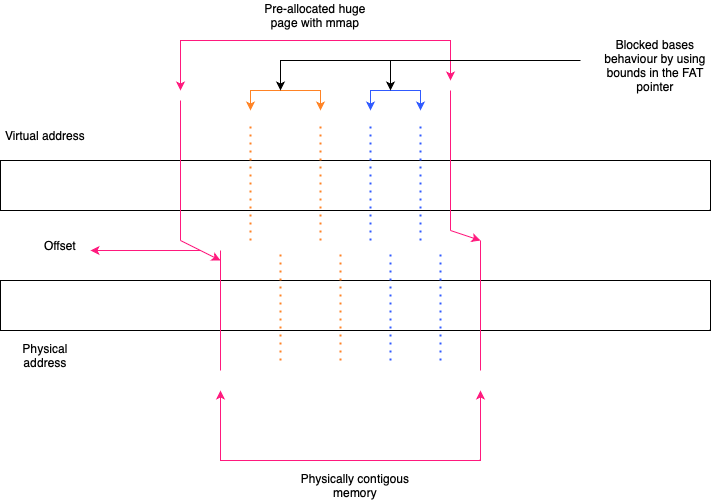
\includegraphics[width=.9\linewidth]{diagram/AllocationOverview24.png}
\caption{\label{fig:org4c237f8}Range of memory}
\end{figure}

Integrating range bounds directly into FAT-pointers enables the architecture 
to enforce memory access restrictions at the pointer level thus allowing 
tracking of memory ranges on a pointer level. In this implementation, memory ranges are established using
bounds encoded within the FAT-pointer, adhering to the CHERI
128-bit bounds compression scheme\cite{woodruff_cheri_2019}.

Figure \ref{fig:RangeOfMemory} illustrates a straightforward use-case in which the dark pink line represents a single, 
large contiguous memory area, or huge page. Within this huge page, the orange and blue lines indicate 
two separate memory allocations equivalent to invoking malloc twice to allocate memory in distinct regions. 
This scenario simulates a block-based memory allocator operating within the confines of the huge page. 
The allocations leverage the bounds encoded in the FAT-pointer, ensuring tracking and efficient 
management of the allocated memory regions. By using the FAT-pointer bounds, this method maintains the 
integrity and contiguity of the allocated blocks within the huge page.

\subsection{Instrumenting Block-Based Allocators with Physically Contiguous Memory}
\label{sec:org56b5427}
\begin{figure}[htbp]
\centering
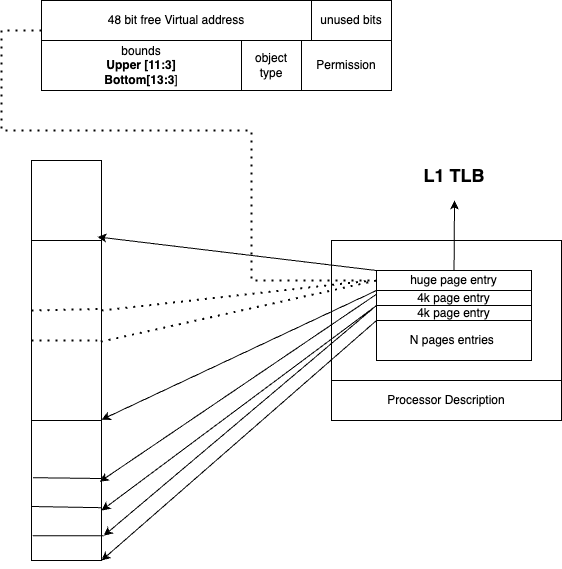
\includegraphics[width=.9\linewidth]{diagram/hugepages.drawio.png}
\caption{\label{fig:org538adae}Fat-pointer Address Translations using huge pages}
\end{figure}

hierarchical structures, to translate virtual addresses to physical addresses. This approach requires multiple entries to handle various
memory segments, leading to increased overhead and complexity
in address translation. Conversely, the current approach stream-
lines this process by using a single TLB entry to translate multiple
addresses within a contiguous memory range. This reduces the
number of required TLB entries, simplifying the translation process
and improving efficiency. By consolidating address translations into
a single TLB entry, this method minimizes the overhead associated
with managing numerous TLB entries and leverages the bounds
encoded within the FAT-pointer for efficient memory tracking and
access. This approach allows for precise and efficient memory management within the allocated huge page.

\begin{itemize}
\item\relax [ ]: Figure \ref{fig:HugePages} illustrates a use case of a huge page to ensure that the
\end{itemize}

\subsection{Implementation}
\label{sec:orgf762315}
The software stack is based on CHERIBSD, selected because ARM officially supports Morello's performance 
counters on this operating system. The setup includes a C program that 
is linked to the prototype memory allocator or to various memory allocators being benchmarked. This linkage can occur in two ways: either as a shared object file during compile time 
for larger allocators, or as a header file for smaller allocators, ensuring flexibility 
in memory management.

This integration ensures that the memory allocation process is optimized for performance, leveraging the contiguity 
of memory blocks and the capabilities provided by the CHERI architecture and the Morello platform. By using the 
contigmem driver and the custom mmap function, the system achieves efficient memory allocation and tracking, 
crucial for the high-performance needs of the application.

\begin{itemize}
\item[{$\square$}] Requires rewrite
\end{itemize}
\subsubsection{kernel module}
\label{sec:org94a3383}
The custom mmap function is tailored to ensure physically contiguous memory is allocated. This allocation is a key component 
of this system. The custom mmap function is interfaced to the contigmem driver, which has been modified from the DPDK library 
. The contigmem driver is essential for managing large contiguous 
memory blocks and is loaded during the system boot process. It reserves a huge page of arbitrary size, with the 
size parameter set based on the requirements of the conducted experiments.

\bibliographystyle{IEEEtran}
\bibliography{FATPointer.bib}
\end{document}